\chapter*{Manual d'usuari}
\label{cha:userguide}

\section{Casa de l'usuari}
\label{sec:home}
En el dashboard es poden veure dues seccions. Les matrius creades per tu i els trainings creats per tu. Actualment no es poden compartir propietat de matrius. Es a dir, una sola persona(el propietari/creador) solament pot editar la matriu. Per poder solventar aquest trau, existeix la possibilitat de clonar una matriu.
\begin{figure}[h!]
  \centering
  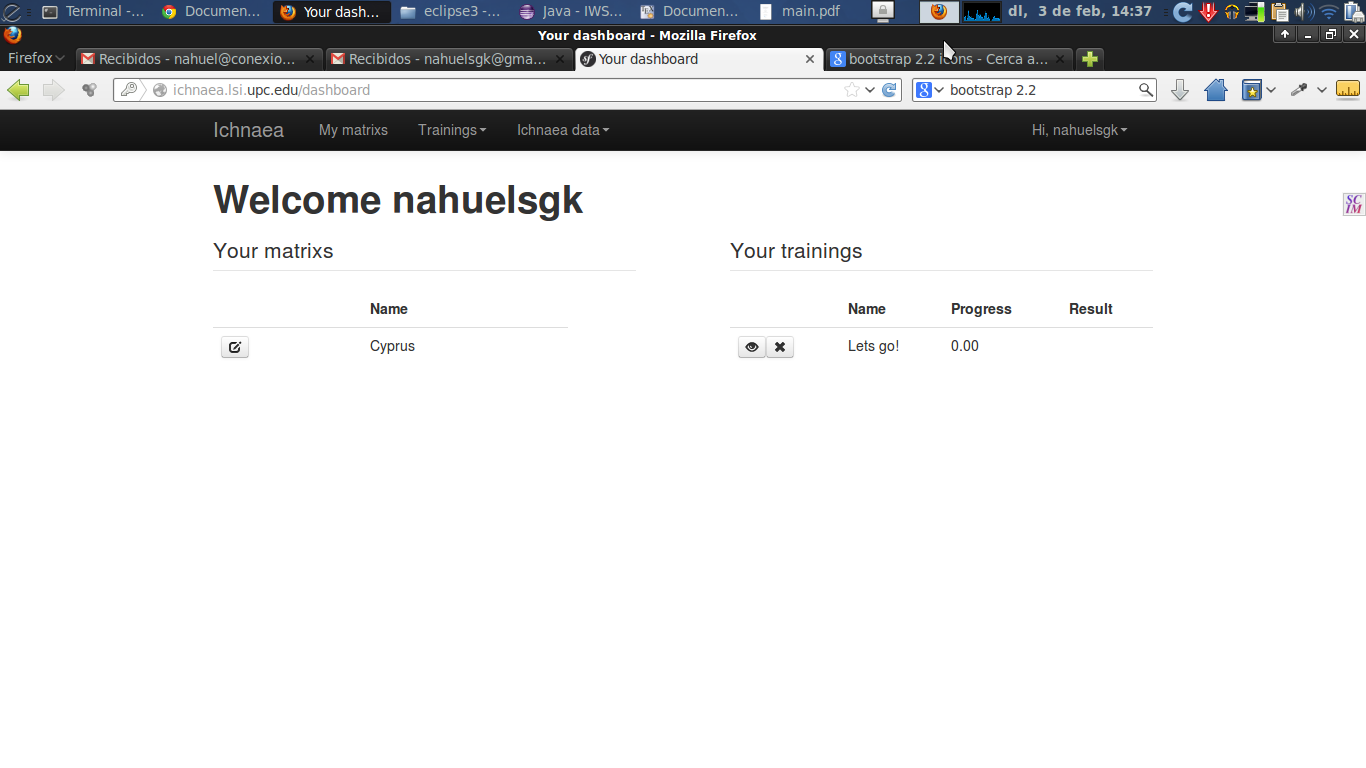
\includegraphics[scale=0.2]{img/userguide/dashboard.png}
  \caption{Casa de l'usuari}
  \label{fig:placement}
\end{figure} 
Al llistat de la esquerra pots veure les matrius que ets propietari. I amb la icona de edici\´{o} pots anar a la pantalla de configuraci\´{o}.
Al llistat de la dreta pots veure els trainings que has llençat.  \´{E}s un llistat de X columnes on:
\begin{itemize}
\item Operacions
 \begin{itemize}
 \item La icona de l'ull es per anar a la pantalla de visualitzaci\´{o} del training.
 \item La icona de X, \´{e}s per esborrar el training.
 \end{itemize}
\item Nom del training
\item Nom de la matriu entrenada
\item Status. Actualment \´{e}s 0 o 1. Es a dir, acabada de entrenar o no. Ichnaea encara no dona status parcials de quan temps li queda per acabar o quan porta.
\end{itemize}

\section{Crear una matriu desde un csv}
\label{sec:create_matrix}
Desde el menu superior "IchnaeaData > New matrix", es pot pujat una nova matriu en format csv. El format csv es compatible amb les programaris de ofim\`{a}tica m\´{e}s habituals como Microsoft Excel o Libreoffice.
El format de la matriu \´{e}s important que sigui el seg\¨{u}ent.
\begin{center}
    \begin{tabular}{ | l | l | l | p{5cm} |}
    \hline
    Cel.la bu\¨{i}da & Alias de la columna & .... & ORIGIN \\ \hline
    Nom de la sample & Valor de la sample  & .... & Origen de la sample \\ \hline
    S01-10-20        & 0,000145            & .... & Human \\ \hline
    \hline
    \end{tabular}
\end{center}
On:
\begin{itemize}
\item Alias de la columna: \´{e}s un nom qualsevol per identificar la columna
\item Valor de la sample: \´{e}s el valor de la mostra per la columna(variable)
\item Nom de la sample: \'{e}s un identificador de la mostra
\end{itemize}
En la pantalla, es pot seleccionar un fitxer csv i pujar'ho. Seguidament, es podr\`{a} establir la relaci\´{o} de la variable real de la columna i quin conjunt de season per defecte usa. 

\section{Configurar una matriu}
\label{sec:configure_matrix}
Per accedir a configurar una matriu, has d'anar a la teva pantalla de inici. Es pot accedir desde "My Matrix" al menu superior. 
Desde la interficie de configuraci\´{o} es pot configurar:
- Donar un alias a la columna
- Asociar una columna a una variable
- Seleccionar un conjunt de seasons de la variable
- Donar nom a un sample
- Donar una data a un sample
- Donar un origen a un sample

\section{Clonar una matriu}
Desde el llistat menu "Ichnaea Data > View Matrix", podem accedir al llistat de variables del sistema. Amb la icona etiquetada com "Clone the matrix", podem clonar una matriu sencera configurada. No es copien els trainings.
\begin{figure}[h!]
  \centering
  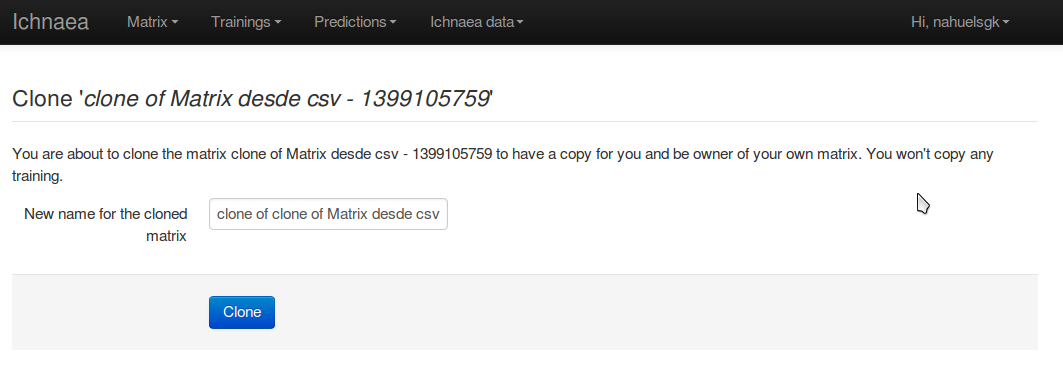
\includegraphics[scale=0.2]{img/userguide/clone_matrix.png}
  \caption{Llistat de matrius}
  \label{fig:placement}
\end{figure}
Fent click a la icona de clonar, anem al formulari que suggereix un nom per identificar-la.
\begin{figure}[h!]
  \centering
  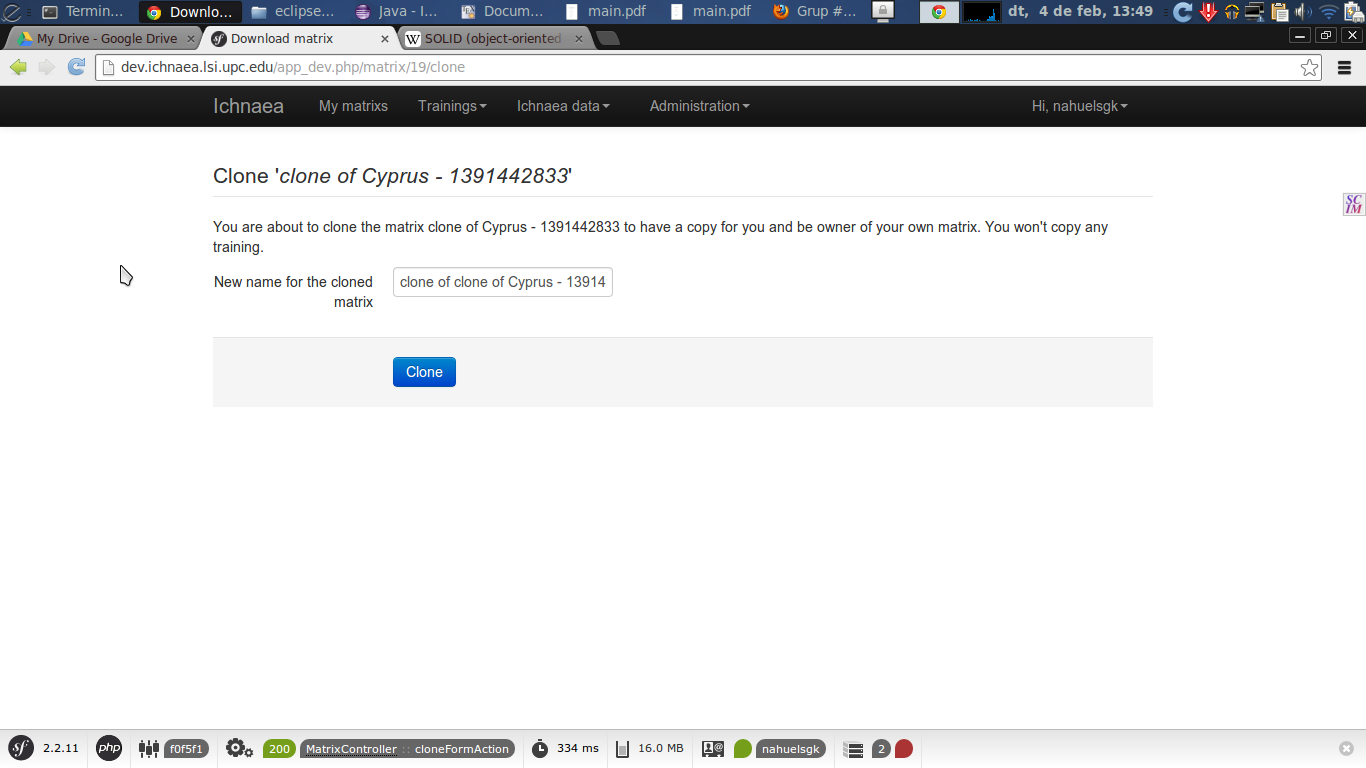
\includegraphics[scale=0.2]{img/userguide/clone_matrix-2.png}
  \caption{Llistat de matrius}
  \label{fig:placement}
\end{figure}
Acceptant, es clona la matriu i anem a la interficie de configuraci\´{o}.


\section{Crear una variable}
Funcionalitat per administradors.

\section{Crear un conjunt de season}

\section{Modificar o afegir m\´{e}s season a una variable}

\section{Crear un training}
Per crear un training s'ha de accedir al menu superior "Trainings > Create a training". Desde el llistat de matrius del sistema, amb la icona de la "carretera", es pot accedir al formulari de creaci\´{o} de trainings.
El training cont\´{e} un nom i una descripci\´{o}. Es poden seleccionar quines columnes vols entrenar de la matriu. 
El origen-versus, es un llistat de la variable origen de la matriu. Si es selecciona el valor "All versus all", el training ser\´{a} tots contra tots. Si \´{e}s selecciona un origen concret, el training es far\´{a}
Si la creaci\´{o} \´e{s} correcte, les dades s'enviaran a la cua de procesos i la aplicaci\´{o} es redirigir\´{a} la pantalla de visualitzaci\´{o} de trainings.

\section{Visualitzar un training}
Desde la casa de l'usuari, es pot veure els teus trainings i en quin estadi es troben. Amb la icona "ull", pots accedir a visualitzar la informaci\´{o} del training.
Una vegada creat es pot veure:
\begin{itemize}
\end{itemize}

\section{Crear una matriu de predicci\'{o}}
Desde la casa de l'usuari, es pot veure els teus trainings i en quin estadi es troben. Amb la icona "Quadradets"


